\begin{frame}[fragile]{Relational Algebra: Select}
\begin{columns}

% ----- COLUMN 1 -----
\column{0.3\textwidth}
\textbf{R(a\_id, b\_id)}

\tiny
\begin{tabular}{ll}
\toprule
a\_id & b\_id \\
\midrule
a1 & 101 \\
a2 & 102 \\
a2 & 103 \\
a3 & 104 \\
\bottomrule
\end{tabular}

% ----- COLUMN 2 -----
\column{0.3\textwidth}
$\sigma_{a\_id = \text{'a2'}}(R)$

\tiny
\begin{tabular}{ll}
\toprule
a\_id & b\_id \\
\midrule
a2 & 102 \\
a2 & 103 \\
\bottomrule
\end{tabular}

% ----- COLUMN 3 -----
\column{0.4\textwidth}
\begin{lstlisting}[language=SQL]
SELECT * FROM R
WHERE a_id='a2' 
  AND b_id>102;
\end{lstlisting}

\end{columns}
\end{frame}



% --- PAGE 44 ---
\begin{frame}[fragile]{Relational Algebra: Projection}
    Generate a relation with tuples that contains only the specified attributes.
    \begin{itemize}
        \item $\rightarrow$ Rearrange attributes’ ordering.
        \item $\rightarrow$ Remove unwanted attributes.
        \item $\rightarrow$ Manipulate values to create derived attributes.
    \end{itemize}
    \vspace{1em}
    \textbf{Syntax:} $\Pi_{A1,A2,\dots,An}(R)$
    \vspace{1em}
    \begin{columns}
        \column{0.5\textwidth}
        $\Pi_{b\_id-100,a\_id}(\sigma_{a\_id='a2'}(R))$
        \column{0.5\textwidth}
        \begin{lstlisting}[language=SQL]
SELECT b_id-100, a_id
FROM R WHERE a_id = 'a2';
        \end{lstlisting}
    \end{columns}
\end{frame}

% --- PAGE 45 ---
\begin{frame}[fragile]{Relational Algebra: Union}
    Generate a relation that contains all tuples that appear in either only one or both input relations.
    \vspace{1em}
    \textbf{Syntax:} $(R \cup S)$
    \vspace{1em}
    \begin{columns}
        \column{0.5\textwidth}
        \begin{itemize}
            \item Standard set algebra rules apply.
        \end{itemize}
        \column{0.5\textwidth}
        \begin{lstlisting}[language=SQL]
(SELECT * FROM R)
UNION
(SELECT * FROM S);
        \end{lstlisting}
    \end{columns}
\end{frame}

% --- PAGE 46 ---
\begin{frame}[fragile]{Relational Algebra: Intersection}
    Generate a relation that contains only the tuples that appear in both of the input relations.
    \vspace{1em}
    \textbf{Syntax:} $(R \cap S)$
    \vspace{1em}
    \begin{columns}
        \column{0.5\textwidth}
        \textbf{R} (a1, a2, a3) \\ \textbf{S} (a3, a4, a5) \\
        $\rightarrow$ Result: (a3)
        \column{0.5\textwidth}
        \begin{lstlisting}[language=SQL]
(SELECT * FROM R)
INTERSECT
(SELECT * FROM S);
        \end{lstlisting}
    \end{columns}
\end{frame}

% --- PAGE 47 ---
\begin{frame}[fragile]{Relational Algebra: Difference}
    Generate a relation that contains only the tuples that appear in the first and not the second of the input relations.
    \vspace{1em}
    \textbf{Syntax:} $(R - S)$
    \vspace{1em}
    \begin{columns}
        \column{0.5\textwidth}
        \textbf{R} (a1, a2, a3) \\ \textbf{S} (a3, a4, a5) \\
        $\rightarrow$ Result: (a1, a2)
        \column{0.5\textwidth}
        \begin{lstlisting}[language=SQL]
(SELECT * FROM R)
EXCEPT
(SELECT * FROM S);
        \end{lstlisting}
    \end{columns}
\end{frame}

% --- PAGE 48 ---
\begin{frame}[fragile]{Relational Algebra: Product}
    Generate a relation that contains all possible combinations of tuples from the input relations.
    \vspace{1em}
    \textbf{Syntax:} $(R \times S)$
    \vspace{1em}
    \begin{lstlisting}[language=SQL]
SELECT * FROM R CROSS JOIN S;
SELECT * FROM R, S;
    \end{lstlisting}
\end{frame}

% --- PAGE 49 ---
\begin{frame}{Relational Algebra: Join}
    Generate a relation that contains all tuples that are a combination of two tuples (one from each input relation) with a common value(s) for one or more attributes.
    \vspace{1em}
    \textbf{Syntax:} $(R \bowtie S)$
\end{frame}

% --- PAGE 50-52 (Join Animations) ---
\begin{frame}[fragile]{Relational Algebra: Join (Examples)}
    \begin{columns}
        \column{0.5\textwidth}
        \textbf{R(a\_id, b\_id)}
        \begin{table}\tiny \begin{tabular}{ll} a1 & 101 \\ a2 & 102 \\ a3 & 103 \end{tabular} \end{table}
        \textbf{S(a\_id, b\_id, val)}
        \begin{table}\tiny \begin{tabular}{lll} a3 & 103 & XXX \\ a4 & 104 & YYY \\ a5 & 105 & ZZZ \end{tabular} \end{table}
        
        \column{0.5\textwidth}
        \textbf{Result $(R \bowtie S)$:}
        \begin{table}\tiny \begin{tabular}{lll} a3 & 103 & XXX \end{tabular} \end{table}
        
        \begin{lstlisting}[language=SQL, basicstyle=\tiny\ttfamily]
SELECT * FROM R NATURAL JOIN S;
SELECT * FROM R JOIN S USING (a_id, b_id);
SELECT * FROM R JOIN S ON R.a_id = S.a_id;
        \end{lstlisting}
    \end{columns}
\end{frame}

% --- PAGE 53 ---
\begin{frame}{Relational Algebra: Extra Operators}
    \begin{itemize}
        \item Rename ($\rho$)
        \item Assignment ($R \leftarrow S$)
        \item Duplicate Elimination ($\delta$)
        \item Aggregation ($\gamma$)
        \item Sorting ($\tau$)
        \item Division ($R \div S$)
    \end{itemize}
\end{frame}

% --- PAGE 54 ---
\begin{frame}{Observation}
    Relational algebra defines an ordering of the high level steps of how to compute a query.
    \begin{itemize}
        \item $\rightarrow$ Example: $\sigma_{b\_id=102}(R \bowtie S)$ vs. $(R \bowtie (\sigma_{b\_id=102}(S)))$
    \end{itemize}
    \vspace{1em}
    A better approach is to state the high-level answer that you want the DBMS to compute.
    \begin{itemize}
        \item $\rightarrow$ Example: Retrieve the joined tuples from R and S where b\_id equals 102.
    \end{itemize}
\end{frame}

% --- PAGE 55 ---
\begin{frame}[fragile]{Relational Model: Queries}
    The relational model is independent of any query language implementation.
    \begin{itemize}
        \item SQL is the de facto standard (many dialects).
    \end{itemize}
    \vspace{1em}
    \begin{columns}
        \column{0.5\textwidth}
        \begin{lstlisting}[language=Python]
for line in file:
 record = parse(line)
 if record[0] == "GZA":
  print(int(record[1]))
        \end{lstlisting}
        \column{0.5\textwidth}
        \begin{lstlisting}[language=SQL]
SELECT year FROM artists
WHERE name = 'GZA';
        \end{lstlisting}
    \end{columns}
\end{frame}

% --- PAGE 56 ---
\begin{frame}{Data Models}
    \begin{itemize}
        \item \textbf{Relational} $\leftarrow$ This Course
        \item Key/Value
        \item Graph
        \item Document / JSON / XML / Object
        \item Wide-Column / Column-family
        \item Array (Vector, Matrix, Tensor)
    \end{itemize}
\end{frame}

% --- PAGE 57 ---
\begin{frame}{Data Models}
    \begin{itemize}
        \item Relational
        \item Key/Value
        \item Graph
        \item \textbf{Document / JSON / XML / Object} $\leftarrow$ Leading Alternative
        \item Wide-Column / Column-family
        \item \textbf{Array (Vector, Matrix, Tensor)} $\leftarrow$ New Hotness
    \end{itemize}
\end{frame}

% --- PAGE 58 ---
\begin{frame}{Document Data Model}
    A collection of record documents containing a hierarchy of named field/value pairs.
    \begin{itemize}
        \item $\rightarrow$ A field’s value can be either a scalar type, an array of values, or another document.
        \item $\rightarrow$ Modern implementations use JSON. Older systems use XML or custom object representations.
    \end{itemize}
    \vspace{1em}
    Avoid “relational-object impedance mismatch” by tightly coupling objects and database.
    \centering
    
\includegraphics[height=1.5cm]{extracted_p58_1_image.png} % MongoDB Logo
    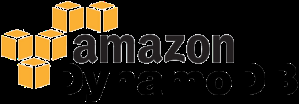
\includegraphics[height=1.5cm]{extracted_p58_2_image.png} % CouchDB Logo
\end{frame}

% --- PAGE 59 & 60 ---
\begin{frame}{Document Data Model (Relational Version)}
    \centering
    \textbf{Artist} $\bowtie$ \textbf{ArtistAlbum} $\bowtie$ \textbf{Album}
    \vspace{1em}
    \\
    $R1(id,\dots)$ \hspace{1em} $R2(artist\_id,album\_id)$ \hspace{1em} $R3(id,\dots)$
\end{frame}

% --- PAGE 61 & 62 ---
\begin{frame}[fragile]{Document Data Model (JSON vs Code)}
    \begin{columns}
        \column{0.5\textwidth}
        \textbf{Document / JSON}
        \begin{verbatim}
{
 "name": "GZA",
 "year": 1990,
 "albums": [
  {
   "name": "Liquid Swords",
   "year": 1995
  },
  ...
 ]
}
        \end{verbatim}
        \column{0.5\textwidth}
        \textbf{Application Code (Java/C++)}
        \begin{verbatim}
class Artist {
  int id;
  String name;
  int year;
  Album albums[];
}
        \end{verbatim}
    \end{columns}
\end{frame}

% --- PAGE 63 & 64 ---
\begin{frame}{Vector Data Model}
    One-dimensional arrays used for nearest-neighbor search (exact or approximate).
    \begin{itemize}
        \item $\rightarrow$ Used for semantic search on embeddings generated by ML trained transformer models (think ChatGPT).
        \item $\rightarrow$ Native integration with modern ML tools and APIs (e.g., LangChain, OpenAI).
    \end{itemize}
    At their core, these systems use specialized indexes to perform NN searches quickly.
    \vspace{1em}
    \centering
    
\includegraphics[height=1cm]{extracted_p63_1_image.png} % Pinecone
    
\includegraphics[height=1cm]{extracted_p63_2_image.png} % Weaviate
    
\includegraphics[height=1cm]{extracted_p63_3_image.png} % Qdrant
    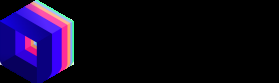
\includegraphics[height=1cm]{extracted_p63_4_image.png} % Milvus
\end{frame}

% --- PAGE 65 ---
\begin{frame}{Vector Data Model}
    \centering
    
\includegraphics[width=0.8\textwidth]{extracted_p65_1_image.png}
    % Diagram: Text -> Embeddings -> Vector Index (HNSW)
\end{frame}

% --- PAGE 66 ---
\begin{frame}{Vector Data Model}
    \centering
    
\includegraphics[width=0.8\textwidth]{extracted_p66_1_image.png}
    % Diagram: Query -> Transformer -> Vector -> Search
\end{frame}

% --- PAGE 67 ---
\begin{frame}{Vector Data Model}
    \centering
    
\includegraphics[width=0.8\textwidth]{extracted_p67_1_image.png}
    % Diagram: Full flow to Ranked List of Ids
\end{frame}

% --- PAGE 68 ---
\begin{frame}{Conclusion}
    \begin{itemize}
        \item Databases are ubiquitous.
        \item Relational algebra defines the primitives for processing queries on a relational database.
        \item We will see relational algebra again when we talk about query optimization + execution.
    \end{itemize}
\end{frame}

% --- PAGE 69 ---
\begin{frame}{Next Class}
    \Large
    \textbf{Modern SQL}
    \vspace{1em}
    \normalsize
    \begin{itemize}
        \item $\rightarrow$ Make sure you understand basic SQL before the lecture.
    \end{itemize}
\end{frame}

% --- PAGE 70 ---
\begin{frame}[fragile]{Ask Andy Anything}
    \begin{itemize}
        \item Questions about database industry?
        \item Questions about database jobs?
        \item Questions about database systems?
    \end{itemize}
\end{frame}